\noindent \textbf{\large Lemma \ref{lem:liq_revenue}}
\begin{proof}
We take the expectation of fee revenues over the size of private value shocks $\delta$ and obtain:
\begin{align}
    \mathbb{E}\text{ProfitLiq}_{i,k}&=2q_i v f_k \times \Big\{ \nonumber \\ &\mathbb{P}\left(f_k<\delta \leq (1+f_k)(1+r)^2-1\right) \times \frac{1+r}{r}\mathbb{E} \left[\sqrt{\frac{1+\delta}{1+f_k}}-1 \mid f_k<\delta \leq (1+f_k)(1+r)^2-1 \right] + \nonumber \\
    &+ \mathbb{P}\left(\delta>(1+f_k)(1+r)^2-1\right) \times \left(1+r\right) \Big\} \nonumber \\
    &=q_i \underbrace{v \frac{f_k (r+1) \left(2 \Delta -r\sqrt{f_k+1} -2 \sqrt{f_k+1}\right)}{\Delta }}_{\equiv \mathcal{L}\left(f_k\right)},
\end{align}
where we define $\mathcal{L}\left(f_k\right)$ as the liquidity yield: i.e., the per-unit profit from liquidity provision in pool $k$.

To explore how the liquidity revenue changes with respect to the pool fee, we differentiate \( \mathcal{L} \) with respect to \( f \):
\begin{equation}
    \frac{\partial{L}\left(f\right)}{\partial f}=-\frac{(r+1) \left(2 \left(-2 \Delta  \sqrt{f+1}+r+2\right)+3 f (r+2)\right)}{4 \Delta  \sqrt{f+1}}.
\end{equation}
Starting with \( f = 0 \) and given that \( \Delta > 1 + r \) (by Assumption \ref{ass:Delta}), the derivative at \( f = 0 \) is positive:
\begin{equation}
   \frac{\partial \mathcal{L}(f)}{\partial f}\bigg|_{f=0} = \frac{(r+1) (2 \Delta - r - 2)}{2 \Delta} > 0, 
\end{equation}
indicating that liquidity revenue increases with pool fee at this point. The derivative has roots:
\begin{equation}
f_{1,2} = \frac{-6 (r+2)^2 + 8 \Delta^2 \pm 4 \sqrt{4 \Delta^4 + 3 \Delta^2 (r+2)^2}}{9 (r+2)^2},    
\end{equation}
where the smallest root \( f_1 \) is negative and therefore not relevant. We need to show that the largest root \( f_2 \) is always positive, defining the threshold \( \overline{f} \).

For this, consider the numerator of $f_2$, labeled \( g(r, \Delta) \):
\[
g(r, \Delta) = 8 \Delta^2 + 4 \sqrt{4 \Delta^4 + 3 \Delta^2 (r+2)^2} - 6 (r+2)^2.
\]
This function has three roots in \( r \), all of which are negative: \( r = -2 \), \( r = -2(1 + \Delta) \), and \( r = 2(\Delta - 1) \). Since these roots are negative, for \( r \geq 0 \), \( g \) does not change sign and it is sufficient to examine \( g(0, \Delta) \):
\begin{equation}
    g(0, \Delta) = 8 \Delta^2 + 4 \sqrt{\Delta^2 (\Delta^2 + 3)} - 6.
\end{equation}
This is positive for any \( \Delta \geq 1 \), confirming that the largest root \( f_2 \) is positive and hence, \( \overline{f} \) exists and is positive. This completes the proof that the liquidity revenue increases with the pool fee until \( \overline{f} \) and decreases with pool fee for $f>\overline{f}$.
\end{proof}


\noindent \textbf{\large Lemma \ref{lem:advsel_fees}}
\begin{proof}
The cost of adverse selection for pool $k$ after evaluating equation \eqref{eq:AScost} is 
\begin{equation}
      \mathcal{A}\left(f_k\right)= v\frac{\left(\Delta -\sqrt{1+f}(1+r)\right) \left(\Delta ^2+\Delta  \sqrt{f+1}\left(1+r\right)+(f+1) (r-2) (r+1)\right)+(f+1)^{3/2} r^2 (r+1)}{3 \Delta }.
\end{equation}
We aim to demonstrate that \( \mathcal{A}(f) \) decreases as \( f \) increases. To do this, we calculate the partial derivative of \( \mathcal{A}(f) \) with respect to \( f \):
\begin{equation}
    \frac{\partial \mathcal{A}\left(f\right)}{\partial f}=\frac{(r+1) \left(-2 \Delta  \sqrt{f+1}+f (r+2)+r+2\right)}{2 \Delta  \sqrt{f+1}}<0
\end{equation}
The derivative is negative if $\Delta > \frac{1}{2} \sqrt{1+f} (2+r)$. Given that $\frac{1}{2}(2+r) < 1+r$, it follows that \( \mathcal{A}(f) \) decreases for any \( \Delta > (1+r) \sqrt{1+f} \), consistent with our assumption on \( \Delta \). \end{proof}

\noindent \textbf{\large Proposition \ref{prop:equilibria}}
\begin{proof}

First, consider the case in which \(\eta > \frac{\mathcal{L}\left(l\right)-\mathcal{L}\left(h\right)}{\mathcal{L}\left(l\right)-\mathcal{L}\left(h\right)+\mathcal{A}\left(l\right)-\mathcal{A}\left(h\right)}\) holds. This implies \(\qmg < 0\), and consequently, \(\pi_L - \pi_H < 0\) for all \(q\). Under this scenario, liquidity providers universally favor pool \(H\) over pool \(L\). They supply liquidity on pool \(H\) if and only if their participation constraint is satisfied, that is if \(q_i > \underline{q}_h\).

Conversely, if \(\eta \leq \frac{\mathcal{L}\left(l\right)-\mathcal{L}\left(h\right)}{\mathcal{L}\left(l\right)-\mathcal{L}\left(h\right)+\mathcal{A}\left(l\right)-\mathcal{A}\left(h\right)}\), then \(\qmg \geq 0\), allowing for a fragmented equilibrium. If \(\qmg \geq 0\), then \(\pi_L\) has a steeper slope compared to \(\pi_H\): profit increases more rapidly with liquidity supply in pool \(L\) than in pool $H$. There are two potential outcomes.

\begin{enumerate}
    \item \textbf{Dominance of pool $L$.} If \(0<\qmg < \underline{q}_\ell < \underline{q}_h\), as shown in the left-hand side panel of the diagram below, then the low-fee pool \(L\) captures the entire market share for any \(q_i\) that yields positive profits. The condition $\underline{q}_\ell < \underline{q}_h$ is equivalent to  
    \begin{equation}
        \underline{q}_\ell < \underline{q}_h \Leftrightarrow \frac{\mathcal{C}\left(h\right)}{\mathcal{C}\left(\ell\right)}>\frac{\left(1-\eta\right)\mathcal{L}\left(h\right)-\eta\mathcal{A}\left(h\right)}{\left(1-\eta\right)\mathcal{L}\left(\ell\right)-\eta\mathcal{A}\left(\ell\right)},
    \end{equation}
    which translates to $\eta>\frac{\mathcal{C}\left(\ell\right) \mathcal{L}\left(h\right)-\mathcal{C}\left(h\right) \mathcal{L}\left(\ell\right)}{\mathcal{C}\left(\ell\right) \left[\mathcal{L}\left(h\right)+\mathcal{A}\left(h\right)\right]-\mathcal{C}\left(h\right) \left[\mathcal{L}\left(\ell\right)+\mathcal{A}\left(\ell\right)\right]}$. Since we require $\eta\leq\frac{\mathcal{L}\left(\ell\right)}{\mathcal{L}\left(\ell\right)+\mathcal{A}\left(\ell\right)}$ by Assumption \ref{ass:eta}, it must be that $\mathcal{L}\left(\ell\right)\mathcal{A}\left(h\right)<\mathcal{L}\left(h\right)\mathcal{A}\left(\ell\right)$. 
    
    However, the parameter regions never overlap, ruling out this scenarios: we will show that $\mathcal{L}\left(\ell\right)\mathcal{A}\left(h\right)-\mathcal{L}\left(h\right)\mathcal{A}\left(\ell\right)>0$. To see this, we first note that $\eta \leq \frac{\mathcal{L}\left(l\right)-\mathcal{L}\left(h\right)}{\mathcal{L}\left(l\right)-\mathcal{L}\left(h\right)+\mathcal{A}\left(l\right)-\mathcal{A}\left(h\right)}$ is equivalent to:
    \begin{equation}\label{eq:c9}
        \eta\leq \frac{3 \left(h \left(2 \Delta -\sqrt{h+1} r-2 \sqrt{h+1}\right)-\ell \left(2 \Delta -\sqrt{\ell+1} r-2 \sqrt{\ell+1}\right)\right)}{(r+2) \left(\sqrt{h+1}\left(h-2 \right)-\sqrt{\ell+1}\left(\ell-2\right)\right)},
    \end{equation}
    which implies that $h \left(2 \Delta -\sqrt{h+1} r-2 \sqrt{h+1}\right)-\ell \left(2 \Delta -\sqrt{\ell+1} r-2 \sqrt{\ell+1}\right)>0$ since the denominator is always positive. We use the inequality in \eqref{eq:c9} and obtain that
    \begin{equation}
    \mathcal{L}\left(\ell\right)\mathcal{A}\left(h\right)-\mathcal{L}\left(h\right)\mathcal{A}\left(\ell\right)>\frac{1+r}{6\Delta^2} g,
    \end{equation}
    where 
    \begin{align}
        g&\equiv \underbrace{(1+r) l  \left(2 \Delta-\sqrt{l+1}\left(r+2\right)\right)}_{>0} \times \\
        & \times \left(\left(h-\ell\right)\Delta - (r+2) \left(\sqrt{h+1}-\sqrt{l+1}\right)+\underbrace{h  \left(2 \Delta-\sqrt{h+1}\left(r+2\right)\right)-l  \left(2 \Delta-\sqrt{l+1}\left(r+2\right)\right)}_{>0}\right)>0,
    \end{align}
    given Assumption \ref{ass:Delta} and equation \eqref{eq:c9}. To see that $\left(h-\ell\right)\Delta - (r+2) \left(\sqrt{h+1}-\sqrt{l+1}\right)>0$, we first note the expression increases in $\Delta$ and is therefore larger than $\sqrt{h+1} (r+1) (h-l)+(r+2) \left(\sqrt{l+1}-\sqrt{h+1}\right)$ for $\Delta>\sqrt{1+h}\left(1+r\right)$. The latter expression increases in $h$ and equals zero for $h=\ell$.The latter expression increases in $h$ and equals zero for $h=\ell$.  
    
    Therefore, there are no parameter values for which \(0<\qmg < \underline{q}_\ell < \underline{q}_h\) and \(\eta \leq \frac{\mathcal{L}\left(l\right)-\mathcal{L}\left(h\right)}{\mathcal{L}\left(l\right)-\mathcal{L}\left(h\right)+\mathcal{A}\left(l\right)-\mathcal{A}\left(h\right)}\), which rules out the case of pool $L$ attracting full market share.
    
    \item \textbf{Fragmented Market Equilibrium.} The right-hand side panel depicts the scenario \(\underline{q}_h < \underline{q}_\ell < \qmg\). Here, liquidity providers with \(q_i\) in the range \((\underline{q}_h, \qmg]\) achieve higher positive profits in pool \(H\), while those with \(q_i > \qmg\) obtain larger profits in pool \(L\). The condition $\underline{q}_h < \underline{q}_\ell$ is equivalent to  
    \begin{equation}
        \underline{q}_h \leq \underline{q}_\ell \Leftrightarrow \frac{\mathcal{C}\left(h\right)}{\mathcal{C}\left(\ell\right)}\leq\frac{\left(1-\eta\right)\mathcal{L}\left(h\right)-\eta\mathcal{A}\left(h\right)}{\left(1-\eta\right)\mathcal{L}\left(\ell\right)-\eta\mathcal{A}\left(\ell\right)},
    \end{equation}
    which is always true if $\eta \leq \frac{\mathcal{L}\left(l\right)-\mathcal{L}\left(h\right)}{\mathcal{L}\left(l\right)-\mathcal{L}\left(h\right)+\mathcal{A}\left(l\right)-\mathcal{A}\left(h\right)}$ as seen above.
\end{enumerate}


\begin{center}
    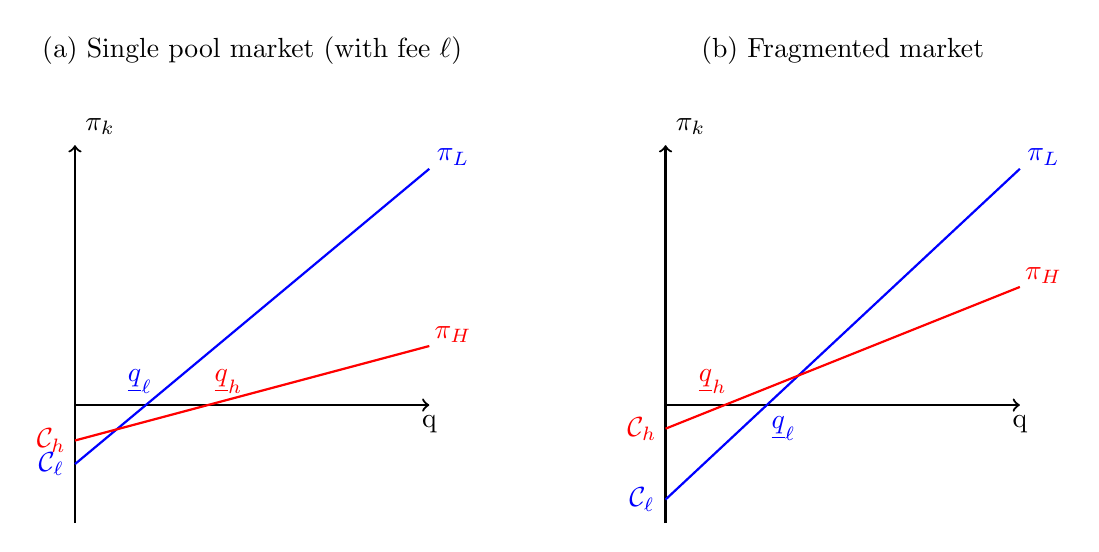
\begin{tikzpicture}[scale=1.5]

    % Axes
    \draw[thick,->] (0,-1) -- (0,2.2) node[anchor=south west] {$\pi_k$};
    \draw[thick,->] (0,0) -- (3,0) node[anchor=north] {q};

    \draw[blue, thick](0,-0.5) -- (3,2);
    \node[blue, align=center] at (0.55,0.2) {$\underline{q}_\ell$};
    \node[blue, align=center] at (3.2,2.1) {$\pi_L$};
    \node[blue, align=center] at (-0.2,-0.5) {$\mathcal{C}_\ell$};

    \draw[red, thick](0,-0.3) -- (3,0.5);
    \node[red, align=center] at (1.3,0.2) {$\underline{q}_h$};
    \node[red, align=center] at (3.2,0.6) {$\pi_H$};
    \node[red, align=center] at (-0.2,-0.3) {$\mathcal{C}_h$};

    \node[black, align=center] at (0.47,-0.3){$\qmg$};

    \node[align=center] at (1.5, 3) {(a) Single pool market (with fee $\ell$)};

    % Axes
    \draw[thick,->] (5,-1) -- (5,2.2) node[anchor=south west] {$\pi_k$};
    \draw[thick,->] (5,0) -- (8,0) node[anchor=north] {q};

    % Lines with negative intercepts but intersecting in the positive quadrant
    \draw[blue, thick](5,-0.8) -- (8,2);
    \node[blue, align=center] at (6,-0.2) {$\underline{q}_\ell$};
    \node[blue, align=center] at (8.2,2.1) {$\pi_L$};
    \node[blue, align=center] at (4.8,-0.8) {$\mathcal{C}_\ell$};

    \draw[red, thick](5,-0.2) -- (8,1);
    \node[red, align=center] at (5.4,0.2) {$\underline{q}_h$};
    \node[red, align=center] at (8.2,1.1) {$\pi_H$};
    \node[red, align=center] at (4.8,-0.2) {$\mathcal{C}_h$};

    % Intersection marker in positive quadrant
    \node[black, align=center] at (6,0.4) {$\qmg$};

        \node[align=center] at (6.5, 3) {(b) Fragmented market};

\end{tikzpicture}
\end{center}

It is crucial to note that configurations where \(\underline{q}_\ell < \qmg < \underline{q}_h\) or \(\underline{q}_h < \qmg < \underline{q}_\ell\) are not feasible, as they would lead to a contradiction where profits are simultaneously positive in one pool and negative in the other at the indifference point \(\qmg\).


\end{proof}

\noindent \textbf{\large Proposition \ref{cor:comp_stat_ms}}
\begin{proof}
We first note that both $\qmg$ and $\underline{q}_h$ scale linearly with $\Gamma$: that is, there exists $Q_t>Q_h>0$ such that $\qmg=\Gamma Q_t$ and $\underline{q}_h=\Gamma Q_h$ where $Q_t$ and $Q_h$ are not functions of $\Gamma$. Next, we compute the partial derivative of $w_\ell$ with respect to $\Gamma$
\begin{equation}
\frac{\partial w_\ell}{\partial \Gamma}=\frac{\Gamma  (Q_h-Q_t) e^{\frac{\Gamma  (Q_h-Q_t)}{\lambda }} (\Gamma  Q_h Q_t+\lambda  (Q_h+Q_t))}{\lambda  (\lambda +\Gamma  Q_h)^2}<0,
\end{equation}
since $Q_h<Q_t$ and all other terms are positive.\end{proof}

\noindent \textbf{\large Proposition \ref{prop:optimality}}
\begin{proof}
The two-pool gains from trade for an $\LT$ with private value $v\left(1+\delta\right)$ are
\begin{align}
    \text{GainsFromTrade}\left(\left\{h,\ell \mid \delta \right\}\right)&=v \delta T_H\min\left\{1,\frac{1+r}{r}\max\left\{0,1-\sqrt{\frac{1+h}{1+\delta}}\right\}\right\}+\nonumber \\&+v \delta T_L\min\left\{1,\frac{1+r}{r}\max\left\{0,1-\sqrt{\frac{1+\ell}{1+\delta}}\right\}\right\}.
\end{align}
We set $h=f$ such that the marginal $\LP$ entering the market is the same as in the single-fee pool; that is, $T_H+T_L=e^{-q_h\lambda}\left(q_h+\lambda\right)$. Since $\min\left\{1,\frac{1+r}{r}\max\left\{0,1-\sqrt{\frac{1+f}{1+\delta}}\right\}\right\}$ decreases in $f$, it follows that:
\begin{align}
    \text{GainsFromTrade}\left(\left\{h,\ell \mid \delta \right\}\right)&\geq v\delta \underbrace{\left(T_H+T_L\right)}_{=e^{-q_h\lambda}\left(q_h+\lambda\right)}\min\left\{1,\frac{1+r}{r}\max\left\{0,1-\sqrt{\frac{1+h}{1+\delta}}\right\}\right\}\\
    &=\text{GainsFromTrade}\left(\left\{h\right\}\mid \delta \right\},
\end{align}
with strict inequality if $\qmg<Q$ such that the low-fee pool attracts a positive mass of $\LP$s. The inequality holds for any $\delta$, and therefore it remains true if we aggregate the gains from trade over the distribution $\LT$ private values. We note that the expected gains from trade per unit of liquidity is
\begin{align}
    &\mathbb{E}\min\left\{1,\frac{1+r}{r}\max\left\{0,1-\sqrt{\frac{1+h}{1+\delta}}\right\}\right\}- \nonumber \\&=\frac{6 \sqrt{f+1} (r+1) \log (r+1)+r \left(2 \left(\Delta ^3-3 \Delta -\sqrt{f+1}\right)+\sqrt{f+1} (f (r+1) (r+2)+r (r+3))\right)}{6 \Delta  r}>0,
\end{align}
which decreases in $f$ since
\begin{align}
    \frac{\partial \mathbb{E}\min\left\{1,\frac{1+r}{r}\max\left\{0,1-\sqrt{\frac{1+h}{1+\delta}}\right\}\right\}}{\partial f}=-\frac{(r+1) ((f+1) r (r+2)-2 \log (r+1))}{4 \Delta  \sqrt{f+1} r}<0.
\end{align}

\end{proof}